\documentclass[11pt]{article}
\usepackage{amsmath,amssymb,amsmath,amsthm,amsfonts}
\usepackage{latexsym,graphicx}
\usepackage{fullpage,color}
\usepackage{url}
\usepackage[pdftex,bookmarks,colorlinks=true,citecolor=blue]{hyperref}
\usepackage{natbib}
\usepackage{graphicx,subfigure}
\usepackage{algorithm}
\usepackage{algorithmic}
\usepackage{listings}
\usepackage{xcolor}
\usepackage{framed}
\usepackage{color}

% \colorlet{shadecolor}{orange!15}
\colorlet{NextBlue}{orange!15!green!50!blue!75}

\numberwithin{equation}{section}

\pagestyle{plain}

\setlength{\oddsidemargin}{0in}
\setlength{\topmargin}{0in}
\setlength{\textwidth}{6.5in}
\setlength{\textheight}{8.5in}

\newtheorem{fact}{Fact}[section]
\newtheorem{question}{Question}[section]
\newtheorem{lemma}{Lemma}[section]
\newtheorem{theorem}[lemma]{Theorem}
\newtheorem{assumption}[lemma]{Assumption}
\newtheorem{corollary}[lemma]{Corollary}
\newtheorem{prop}[lemma]{Proposition}
\newtheorem{claim}{Claim}[section]
\newtheorem{remark}{Remark}[section]
\newtheorem{definition}{Definition}[section]
\newtheorem{prob}{Problem}[section]
\newtheorem{conjecture}{Conjecture}[section]
\newtheorem{property}{Property}[section]

\def\A{{\bf A}}
\def\a{{\bf a}}
\def\B{{\bf B}}
\def\bb{{\bf b}}
\def\C{{\bf C}}
\def\c{{\bf c}}
\def\D{{\bf D}}
\def\d{{\bf d}}
\def\E{{\bf E}}
\def\e{{\bf e}}
\def\F{{\bf F}}
\def\f{{\bf f}}
\def\g{{\bf g}}
\def\h{{\bf h}}
\def\G{{\bf G}}
\def\H{{\bf H}}
\def\I{{\bf I}}
\def\K{{\bf K}}
\def\k{{\bf k}}
\def\LL{{\bf L}}
\def\M{{\bf M}}
\def\m{{\bf m}}
\def\N{{\bf N}}
\def\n{{\bf n}}
\def\PP{{\bf P}}
\def\pp{{\bf p}}
\def\Q{{\bf Q}}
\def\q{{\bf q}}
\def\R{{\bf R}}
\def\rr{{\bf r}}
\def\S{{\bf S}}
\def\s{{\bf s}}
\def\T{{\bf T}}
\def\tt{{\bf t}}
\def\U{{\bf U}}
\def\u{{\bf u}}
\def\V{{\bf V}}
\def\v{{\bf v}}
\def\W{{\bf W}}
\def\w{{\bf w}}
\def\X{{\bf X}}
\def\x{{\bf x}}
\def\Y{{\bf Y}}
\def\y{{\bf y}}
\def\Z{{\bf Z}}
\def\z{{\bf z}}
\def\0{{\bf 0}}
\def\1{{\bf 1}}



\def\AM{{\mathcal A}}
\def\CM{{\mathcal C}}
\def\DM{{\mathcal D}}
\def\EM{{\mathcal E}}
\def\GM{{\mathcal G}}
\def\FM{{\mathcal F}}
\def\IM{{\mathcal I}}
\def\JM{{\mathcal J}}
\def\KM{{\mathcal K}}
\def\LM{{\mathcal L}}
\def\NM{{\mathcal N}}
\def\OM{{\mathcal O}}
\def\PM{{\mathcal P}}
\def\SM{{\mathcal S}}
\def\TM{{\mathcal T}}
\def\UM{{\mathcal U}}
\def\VM{{\mathcal V}}
\def\WM{{\mathcal W}}
\def\XM{{\mathcal X}}
\def\YM{{\mathcal Y}}
\def\RB{{\mathbb R}}
\def\RBmn{{\RB^{m\times n}}}
\def\EB{{\mathbb E}}
\def\PB{{\mathbb P}}

\def\TX{\tilde{\bf X}}
\def\TA{\tilde{\bf A}}
\def\tx{\tilde{\bf x}}
\def\ty{\tilde{\bf y}}
\def\TZ{\tilde{\bf Z}}
\def\tz{\tilde{\bf z}}
\def\hd{\hat{d}}
\def\HD{\hat{\bf D}}
\def\hx{\hat{\bf x}}
\def\nysA{{\tilde{\A}_c^{\textrm{nys}}}}

\def\alp{\mbox{\boldmath$\alpha$\unboldmath}}
\def\bet{\mbox{\boldmath$\beta$\unboldmath}}
\def\epsi{\mbox{\boldmath$\epsilon$\unboldmath}}
\def\etab{\mbox{\boldmath$\eta$\unboldmath}}
\def\ph{\mbox{\boldmath$\phi$\unboldmath}}
\def\pii{\mbox{\boldmath$\pi$\unboldmath}}
\def\Ph{\mbox{\boldmath$\Phi$\unboldmath}}
\def\Ps{\mbox{\boldmath$\Psi$\unboldmath}}
\def\ps{\mbox{\boldmath$\psi$\unboldmath}}
\def\tha{\mbox{\boldmath$\theta$\unboldmath}}
\def\Tha{\mbox{\boldmath$\Theta$\unboldmath}}
\def\muu{\mbox{\boldmath$\mu$\unboldmath}}
\def\Si{\mbox{\boldmath$\Sigma$\unboldmath}}
\def\si{\mbox{\boldmath$\sigma$\unboldmath}}
\def\Gam{\mbox{\boldmath$\Gamma$\unboldmath}}
\def\Lam{\mbox{\boldmath$\Lambda$\unboldmath}}
\def\De{\mbox{\boldmath$\Delta$\unboldmath}}
\def\Ome{\mbox{\boldmath$\Omega$\unboldmath}}
\def\Pii{\mbox{\boldmath$\Pi$\unboldmath}}
\def\varepsi{\mbox{\boldmath$\varepsilon$\unboldmath}}
\newcommand{\ti}[1]{\tilde{#1}}
\def\Ncal{\mathcal{N}}
\def\argmax{\mathop{\rm argmax}}
\def\argmin{\mathop{\rm argmin}}

\def\ALG{{\AM_{\textrm{col}}}}

\def\mean{\mathsf{mean}}
\def\std{\mathsf{std}}
\def\bias{\mathsf{bias}}
\def\var{\mathsf{var}}
\def\sgn{\mathsf{sgn}}
\def\tr{\mathsf{tr}}
\def\rk{\mathrm{rank}}
\def\nnz{\mathsf{nnz}}
\def\poly{\mathrm{poly}}
\def\diag{\mathsf{diag}}
\def\Diag{\mathsf{Diag}}
\def\const{\mathrm{Const}}
\def\st{\mathsf{s.t.}}
\def\vect{\mathsf{vec}}
\def\sech{\mathrm{sech}}
\def\sigmoid{\mathsf{sigmoid}}

\newcommand{\red}[1]{{\color{red}#1}}



\def\argmax{\mathop{\rm argmax}}
\def\argmin{\mathop{\rm argmin}}

\newenvironment{note}[1]{\medskip\noindent \textbf{#1:}}%
        {\medskip}


\newcommand{\etal}{{\em et al.}\ }
\newcommand{\assign}{\leftarrow}
\newcommand{\eps}{\epsilon}

\newcommand{\opt}{\textrm{\sc OPT}}
\newcommand{\script}[1]{\mathcal{#1}}
\newcommand{\ceil}[1]{\lceil #1 \rceil}
\newcommand{\floor}[1]{\lfloor #1 \rfloor}



\lstset{ %
extendedchars=false,            % Shutdown no-ASCII compatible
language=Python,                % choose the language of the code
xleftmargin=1em,
xrightmargin=1em,
basicstyle=\footnotesize,    % the size of the fonts that are used for the code
tabsize=3,                            % sets default tabsize to 3 spaces
numbers=left,                   % where to put the line-numbers
numberstyle=\tiny,              % the size of the fonts that are used for the line-numbers
stepnumber=1,                   % the step between two line-numbers. If it's 1 each line
                                % will be numbered
numbersep=5pt,                  % how far the line-numbers are from the code   %
keywordstyle=\color[rgb]{0,0,1},                % keywords
commentstyle=\color[rgb]{0.133,0.545,0.133},    % comments
stringstyle=\color[rgb]{0.627,0.126,0.941},      % strings
backgroundcolor=\color{white}, % choose the background color. You must add \usepackage{color}
showspaces=false,               % show spaces adding particular underscores
showstringspaces=false,         % underline spaces within strings
showtabs=false,                 % show tabs within strings adding particular underscores
frame=single,                 % adds a frame around the code
%captionpos=b,                   % sets the caption-position to bottom
breaklines=true,                % sets automatic line breaking
breakatwhitespace=false,        % sets if automatic breaks should only happen at whitespace
%title=\lstname,                 % show the filename of files included with \lstinputlisting;
%                                % also try caption instead of title
mathescape=true,escapechar=?    % escape to latex with ?..?
escapeinside={\%*}{*)},         % if you want to add a comment within your code
%columns=fixed,                  % nice spacing
%morestring=[m]',                % strings
%morekeywords={%,...},%          % if you want to add more keywords to the set
%    break,case,catch,continue,elseif,else,end,for,function,global,%
%    if,otherwise,persistent,return,switch,try,while,...},%
}


\begin{document}

%\setlength{\fboxrule}{.5mm}\setlength{\fboxsep}{1.2mm}
%\newlength{\boxlength}\setlength{\boxlength}{\textwidth}
%\addtolength{\boxlength}{-4mm}


\title{Analyzing Federated Learning through an Adversarial Lens}

\author{\textbf{Arjun Nitin \etal}}

%\date{ }

\maketitle

\begin{abstract}
% This lecture note describes synchronous parallel accelerated gradient descent (AGD) for empirical risk minimization ERM.
% We first describe AGD for solving ERM.
% We then show how to parallelize AGD; in particular, we assume there is a central parameter server and the data are partitioned among the worker nodes.
% We finally use Python to write a simulator that mimics synchronous parallel AGD.
Federated learning trains a global model on a server with a multitude of agents. These agents use their local data to train but only share model parameter updates. Federated learning may suffer a new threat, namely model poisoning. This paper introduce this kind of threat and show that ef- fective and stealthy model poisoning attacks are possible, highlighting vulnerabilities in the fed- erated learning setting.

\end{abstract}

\section{Federated Learning} 

It happens when the network is fed an "adversarial example".

\colorbox{orange!15}{Adversarial example}

\begin{itemize}
    \item perturbed input
    \item it looks and feels exactly the same as its untampered copy to a human
    \item it completely throws off the classifier
\end{itemize}

\begin{figure}[!h]
	\centering
	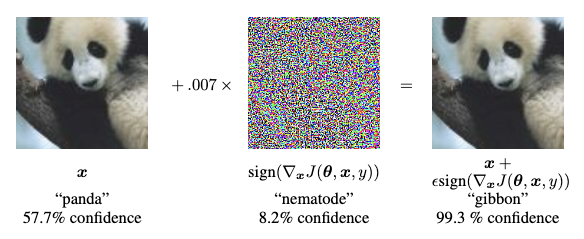
\includegraphics[width=12cm]{figures/evasion.png}
% 	\caption{Illustration of parallel AGD.}
	\label{fig:evasion}
\end{figure}


\section{Why do Adversarial Examples Exist?}

A number of hypotheses:

\begin{enumerate}
    \item Due to low-probability "pockets" in the manifold(i.e. too much non-linearity) and poor regularization~{\cite{szegedy2013intriguing}};
    \item Due to \textit{too much} linearity.(Relu, Sigmoid are basically straight lines in the middle). Accumulate the tiny perturbations of some input into massive difference on the end of the network ~{\cite{goodfellow2014explaining}}.
    \item Tilted boundary(perhaps most commonly adopted hypothesis)~\cite{tanay2016boundary}.The model never fits the data perfectly. There will always be adversarial pockets of inputs that exist between the boundary of the classifier and the actual sub-manifold of sampled data.
    \item Lack of sufficient training data~\cite{schmidt2018adversarially}.
    \item Computational intractability of ever building robust classifiers~\cite{bubeck2018adversarial}.
\end{enumerate}

Adversarial examples are not a bug, they are feature of how neural networks see the world~\cite{ilyas2019adversarial}. And \url{http://gradientscience.org/adv/} is a blog summary of this paper.

\section{Five classes of evasion attacks:}

\begin{enumerate}
    \item Those that use gradients
    \item Those that use confidence scores
    \item Those that use hard labels
    \item Those that use surrogate models
    \item Brute-fore attacks
\end{enumerate}

\colorbox{orange!15}{Gradient-based attacks}

Require access to the model's gradients and are a type of\textbf{ WhiteBox attacks.}

\begin{itemize}
    \item EDA($L_1$ norm)~\cite{chen2018ead}
    \item C\&W($L_2$ norm)~\cite{carlini2017adversarial}
    \item Madry($L_i$ norm)~\cite{madry2017towards}
\end{itemize}

\colorbox{orange!15}{Confidence score attacks}

Use the outputted classification confidence to estimate the gradients of the model, and then perform similar smart optimization to gradient-based attacks above.\textbf{ BlackBox attack}.

\begin{itemize}
    \item ZOO~\cite{chen2017zoo}
    \item SPSA~\cite{uesato2018adversarial}
    \item NES~\cite{ilyas2018black}
\end{itemize}

\colorbox{orange!15}{Hard label}

Rely solely on the label outputted by the model and do not require the confidence scores.

Example in this category: Boundary Attack~\cite{brendel2017decision}.


\colorbox{orange!15}{Surrogate model}

Try to rebuild the target's model(query, guess the architecture and data, take any off-the-shelf image classifier and produce imperfect but functional adversarial examples).

\colorbox{orange!15}{Brute-force attacks}

Use no optimization at all to generate adversarial examples.

\begin{itemize}
    \item Randomly rotating / translating the image~\cite{engstrom2019exploring}
    \item Applying common perturbations~\cite{hendrycks2018benchmarking}
    \item Adding Gaussian noise with large SD~\cite{ford2019adversarial}
\end{itemize}

\section{Defend Against Adversarial Examples}

Two broad categories of defenses:

\begin{enumerate}
    \item formal methods
    \item empirical defenses
\end{enumerate}

\colorbox{orange!15}{formal method}

Attempt every possible scenario. For evasion attacks, try to generate every possible adversarial example within a certain radius of perturbation. They are not cheap and often completely intractable from a computational perspective. Some papers of this:
\begin{itemize}
    \item Reluplex: An Efficient SMT Solver for Verifying Deep Neural Networks
    \item Safety Verification of Deep Neural Networks
    \item Evaluating Robustness of Neural Networks with Mixed Integer Programming
\end{itemize}

\colorbox{orange!15}{empirical defenses}

\begin{enumerate}
    \item Adversarial training
    \item Gradient masking
    \item Input modification
    \item Detection
    \item Extra class
\end{enumerate}

\bibliographystyle{plain}

%\markboth{\bibname}{\bibname}
% \bibliography{bib/decentralized,bib/distributed,bib/system}
\bibliography{bib/decentralized,bib/distributed,bib/system,bib/poison}

\end{document}
